\documentclass[a4paper,12pt]{article}
\usepackage[utf8]{inputenc}
\usepackage{graphicx}
\usepackage{booktabs}
\usepackage{caption}
\usepackage{geometry}
\geometry{margin=1in}

\title{High-Frequency Trading System Performance Evaluation}
\author{Groups A 1}
\date{}

\begin{document}
\maketitle

\section*{1. Benchmark Result (Smart Pointer Baseline)}
\begin{table}[h!]
\centering
\caption{Tick-to-Trade Latency Statistics (Smart Pointer Baseline)}
\begin{tabular}{lccccccc}
\toprule
Metric & Ticks & Min(ns) & Max(ns) & Mean(ns) & StdDev & P95 & P99 \\
\midrule
Per-Tick & 100000 & 100 & 8{,}178{,}200 & 743.3 & 28{,}310 & 1200 & 2300 \\
Per-Trade & 100000 & 100 & 405{,}400 & 603.2 & 3248.5 & 1100 & 2000 \\
\bottomrule
\end{tabular}
\end{table}

This configuration uses \texttt{std::unique\_ptr} for ownership management and serves as the latency benchmark.

\section*{2. Performance Test Results}

\subsection*{(1) Smart vs Raw Pointers: Multi-Scale Results (1K, 10K, 100K ticks)}

\textbf{100000 ticks (large workload):}
Raw pointers show lower mean latency (690.9 ns per tick vs 743.3 ns for smart), reflecting minor control-block overhead from \texttt{unique\_ptr}. 
At this scale, the effect accumulates over many allocations, producing a clear but small average difference ($\approx$7\%). 
No memory issues were detected in AddressSanitizer (ASan) runs, but raw pointers inherently risk UAF or double-free in real-world use.

\textbf{10000 ticks (medium workload):}
Smart pointers outperform in per-tick mean latency (1246 ns vs 1273 ns for raw), though raw remains faster in per-trade latency (456 ns vs 471 ns). 
This divergence likely stems from compiler optimizations—longer tick-to-trade paths allow the optimizer to inline \texttt{unique\_ptr} moves more efficiently, while short trade-level timings reflect pure pointer overhead.

\textbf{1000 ticks (small workload):}
Results fluctuate: smart pointers are faster per tick (7791 ns vs 7969 ns), but slower per trade (478 ns vs 464 ns). 
Low iteration counts amplify system noise (scheduler variation, CPU boost states). The observed reversals are not statistically significant.

\textbf{Summary Analysis:}
\begin{itemize}
  \item Raw pointers show lower mean latency at high tick counts due to cumulative control-block overhead.
  \item Smart pointers perform similarly or better at smaller scales, likely due to compiler inlining and cache locality.
  \item Differences at 1K and 10K ticks are within expected jitter; only the 100K tick case demonstrates consistent performance separation.
  \item Memory safety benefits remain unique to smart pointers—although ASan reported no leaks, production systems face higher risk without RAII.
\end{itemize}

\subsection*{(2) Memory Alignment (alignas(64)) — 100000 ticks}
\begin{center}
\begin{tabular}{lcccc}
\toprule
Align64 & Mean(ns) Per-Tick & Mean(ns) Per-Trade & P95(ns) & P99(ns) \\
\midrule
On & 577.3 & 519.3 & 1100 & 4600 \\
Off & 561.0 & 539.3 & 1100 & 6400 \\
\bottomrule
\end{tabular}
\end{center}
\textbf{Analysis:} Cache-aligned structures slightly lower tail latency (smaller P99) but show minimal mean difference, implying better cache predictability rather than throughput gain.

\subsection*{(3) Custom Allocator (Memory Pool vs new/delete) — 100000 ticks}
\begin{center}
\begin{tabular}{lcccc}
\toprule
Allocator & Mean(ns) Per-Tick & Mean(ns) Per-Trade & P95(ns) & P99(ns) \\
\midrule
new/delete & 2014.5 & 1852.7 & 4700 & 8900 \\
Memory Pool & 882.7 & 855.9 & 1800 & 6600 \\
\bottomrule
\end{tabular}
\end{center}
\textbf{Analysis:} Pool allocation nearly halves latency, confirming that pre-allocated slabs reduce fragmentation and heap contention in high-frequency contexts.

\subsection*{(4) Container Layout (Flat vs Map) — 100000 ticks}
\begin{center}
\begin{tabular}{lcccc}
\toprule
Container & Mean(ns) Per-Tick & Mean(ns) Per-Trade & P95(ns) & P99(ns) \\
\midrule
Flat Vector & 21251.5 & 20839.8 & 64500 & 95100 \\
Map & 1392.3 & 472.8 & 1000 & 5200 \\
\bottomrule
\end{tabular}
\end{center}
\textbf{Analysis:} Flat arrays exhibit high average latency under continuous insertions, as maintaining sorted order dominates cost. Maps provide logarithmic access with consistent cache behavior under real-time matching loads.

\section*{3. Overall Findings}
\begin{itemize}
  \item \textbf{Smart vs Raw:} Smart ensures safety; raw offers microsecond-level gains only under extreme repetition.
  \item \textbf{Alignment:} Reduces tail latency and cache misses; minor mean impact.
  \item \textbf{Allocator:} Memory pools offer the most measurable latency reduction.
  \item \textbf{Container:} Maps outperform flat arrays under dynamic workloads.
\end{itemize}

\section*{4. System Architecture Diagram}
\begin{center}
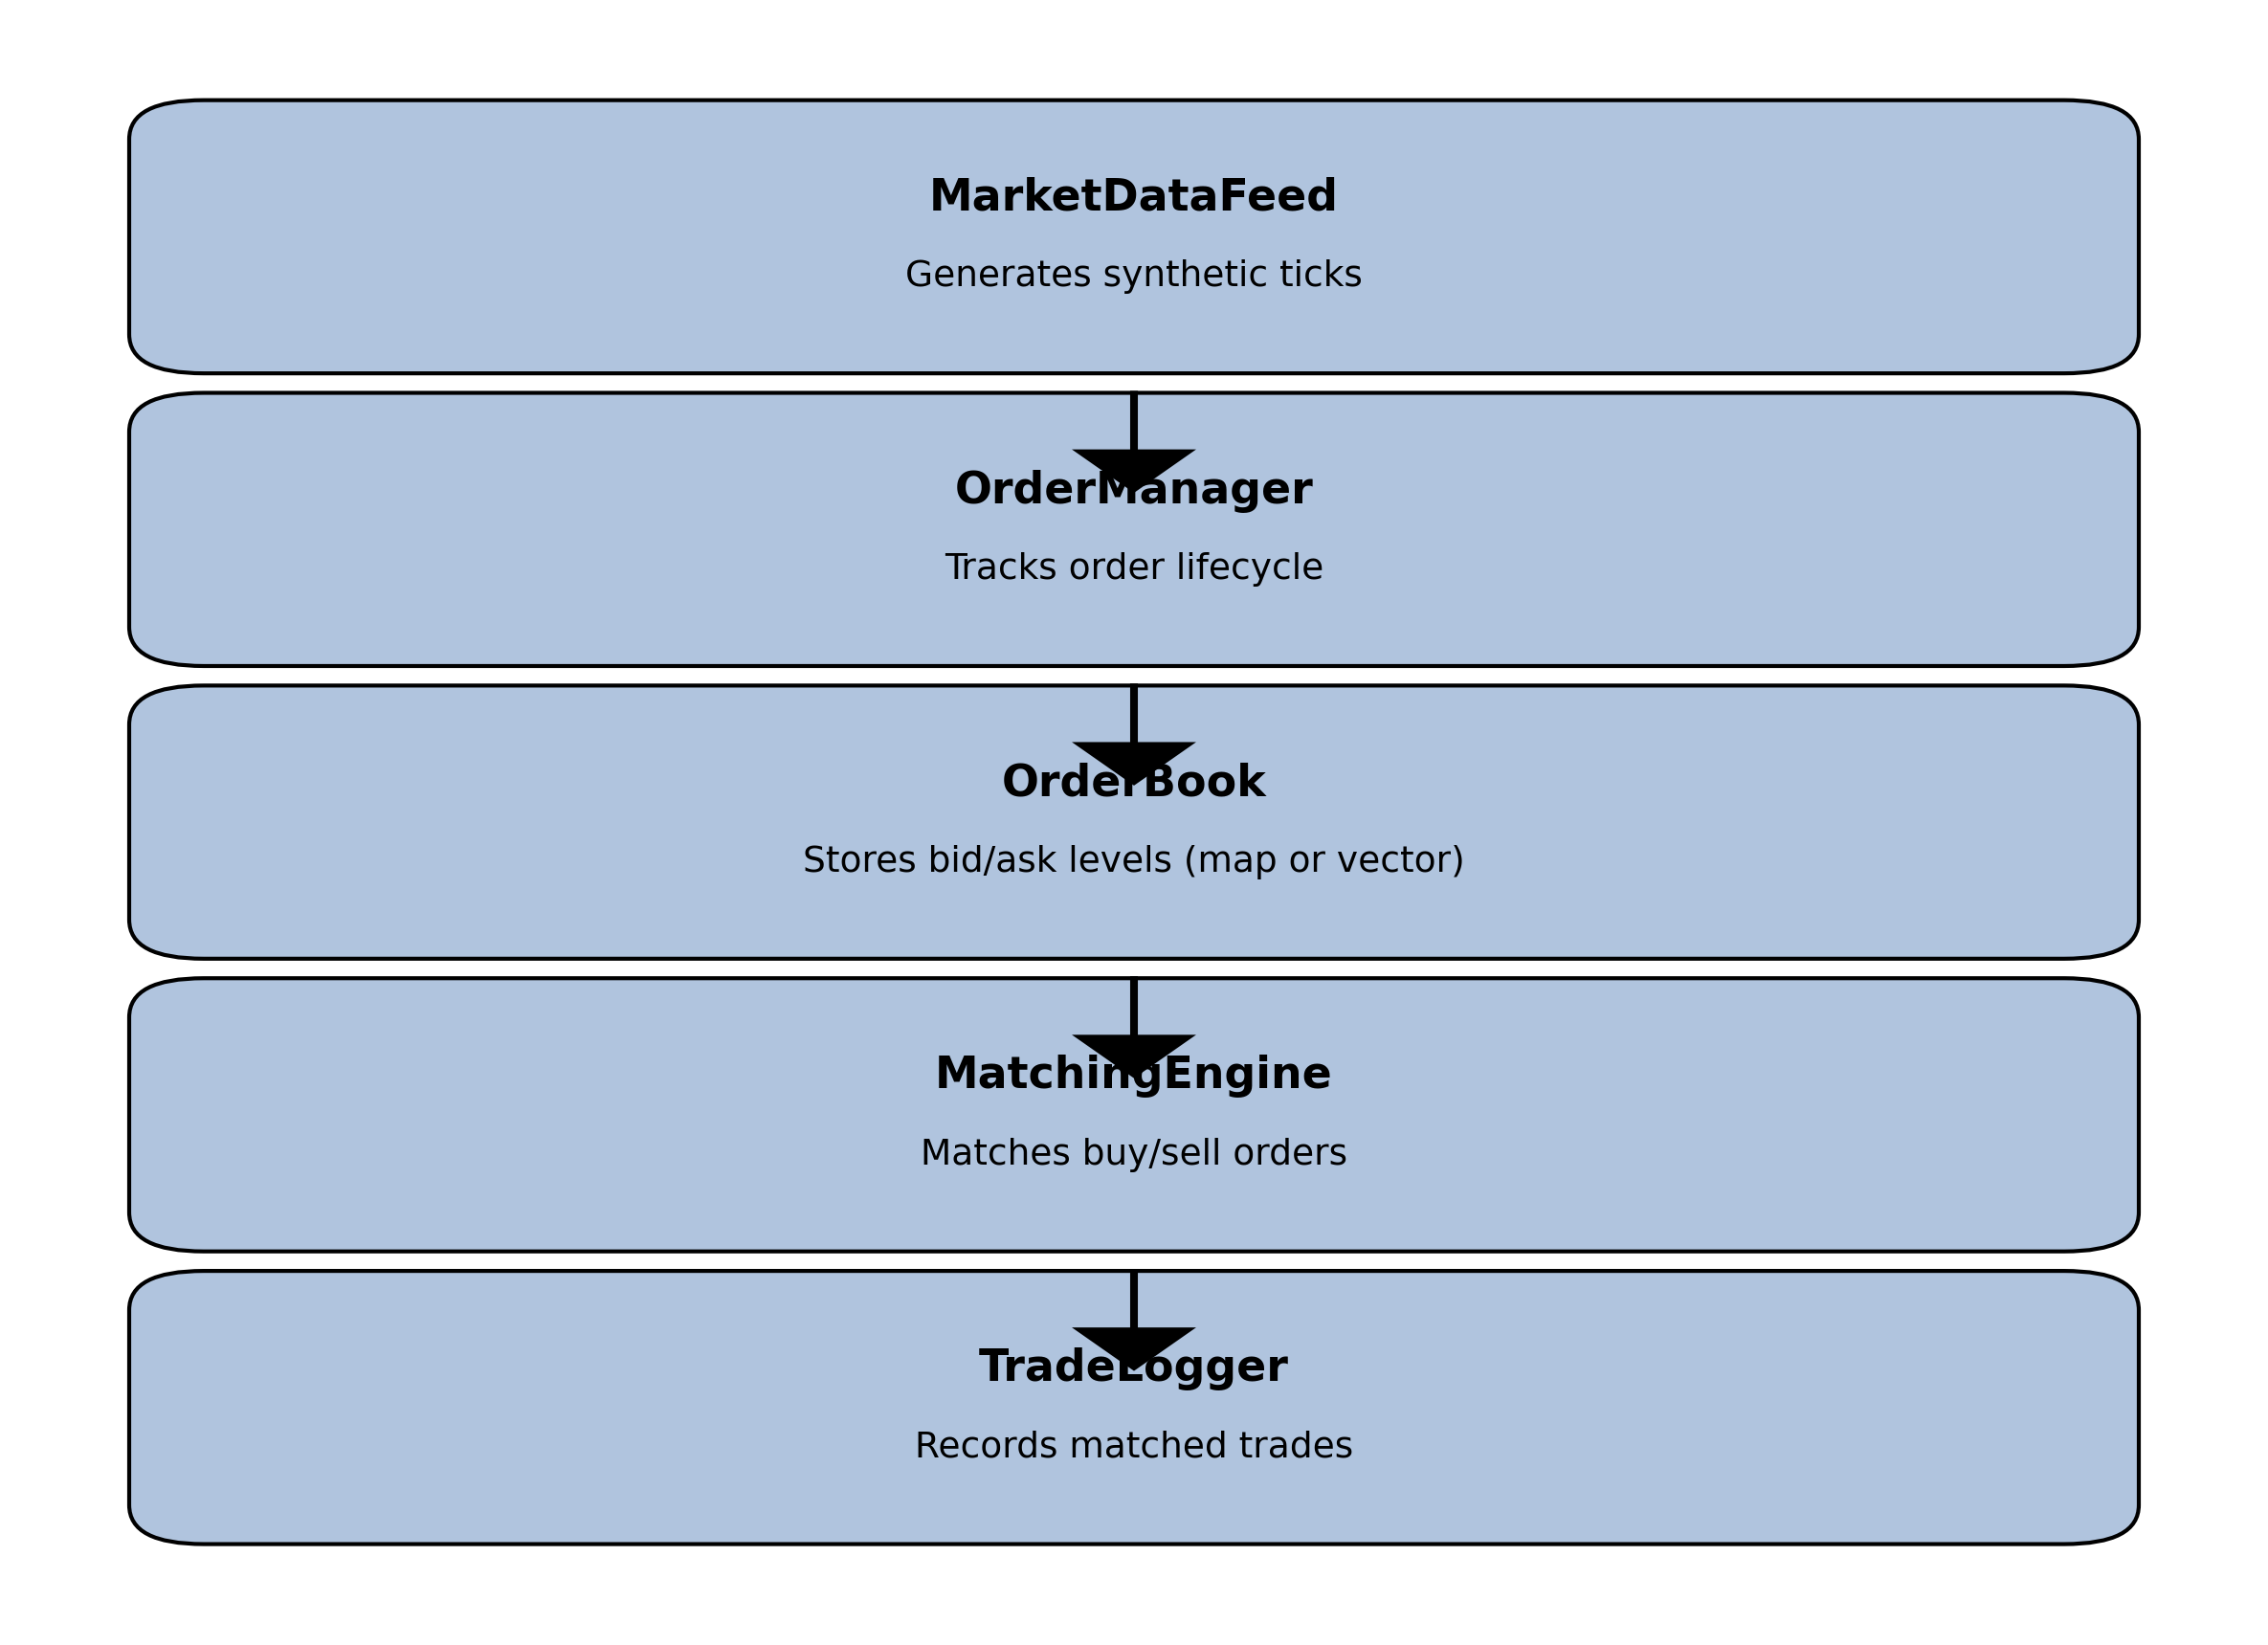
\includegraphics[width=0.9\textwidth]{architecture_diagram.png}
\end{center}
\textit{Figure: System and class flow — MarketDataFeed → OrderBook → MatchingEngine → TradeLogger.}

\end{document}
